%\documentclass[iop]{emulateapj}
\documentclass[aps, pre, onecolumn, nofootinbib, notitlepage, groupedaddress, amsfonts, amssymb, amsmath, longbibliography]{revtex4-1}
\usepackage{tabularx}
\usepackage{graphicx}
\usepackage{hyperref}
\usepackage{xcolor}
\hypersetup{
    colorlinks,
    linkcolor={red!50!black},
    citecolor={blue!50!black},
    urlcolor={blue!80!black}
}
\usepackage{bm}
\usepackage{natbib}
\usepackage{longtable}
\LTcapwidth=0.87\textwidth

\newcommand{\Div}[1]{\ensuremath{\nabla\cdot\left( #1\right)}}
\newcommand{\DivU}{\ensuremath{\nabla\cdot\bm{u}}}
\newcommand{\angles}[1]{\ensuremath{\left\langle #1 \right\rangle}}
\newcommand{\grad}{\ensuremath{\nabla}}
\newcommand{\RB}{Rayleigh-B\'{e}nard }
\newcommand{\stressT}{\ensuremath{\bm{\bar{\bar{\Pi}}}}}
\newcommand{\lilstressT}{\ensuremath{\bm{\bar{\bar{\sigma}}}}}
\newcommand{\nrho}{\ensuremath{n_{\rho}}}
\newcommand{\approptoinn}[2]{\mathrel{\vcenter{
	\offinterlineskip\halign{\hfil$##$\cr
	#1\propto\cr\noalign{\kern2pt}#1\sim\cr\noalign{\kern-2pt}}}}}

\newcommand{\appropto}{\mathpalette\approptoinn\relax}

\newcommand\mnras{{MNRAS}}%

\begin{document}
\author{Evan H. Anders}
\affiliation{Dept. Astrophysical \& Planetary Sciences, University of Colorado -- Boulder, Boulder, CO 80309, USA}
\affiliation{Laboratory for Atmospheric and Space Physics, Boulder, CO 80303, USA}
\author{Benjamin P. Brown}
\affiliation{Dept. Astrophysical \& Planetary Sciences, University of Colorado -- Boulder, Boulder, CO 80309, USA}
\affiliation{Laboratory for Atmospheric and Space Physics, Boulder, CO 80303, USA}
\author{Jeffrey S. Oishi}
\affiliation{Department of Physics and Astronomy, Bates College, Lewiston, ME 04240, USA}
\title{Accelerated convergence of convective simulations using boundary value problems}

\begin{abstract}
We present a method for coupling boundary value problems (BVPs) with initial value problems (IVPs)
in order to achieve thermally converged convective solutions on dynamical timescales, rather than the
long thermal timescale. We study this method in the context of \RB convection. 
We demonstrate that the solution reached by BVP and the
solution reached by a long thermal rundown of the IVP are similar, and demonstrate that this method works at a
large range of supercriticalities.  The BVP method is used to achieve converged solutions at high supercriticality ($10^8$),
and its extensions to more complex scenarios are discussed.
\end{abstract}
\maketitle

\section{Introduction}
\label{sec:intro}
Natural convection occurs in the presence of disparate timescales. Granules on the
solar surface overturn on the order of 10 minutes, whereas deep motions in the Sun at
low Mach number are constrained by the solar rotation rate of $\sim$1 month.  
These dynamical timescales are vastly shorter than the Sun's 
Kelvin-Helmholtz timescale of nearly $3 \times 10^7$ \emph{years} \cite{stix2003}. 
Modern simulations aim to model natural convection
by increasing into the high-Rayleigh-Number (Ra) regime, in which energy transportation occurs on
timescales much larger than dynamical timescales \cite{anders&brown2017}.
In this regime, simulations must pass through a great number
of convective timescales to reach a thermally converged state.
Furthermore, as Ra increases and diffusivities correspondingly decrease, 
motions become more turbulent. To properly resolve these turbulent motions, fine grid meshes
and short timesteps are required; these requirements increase the computational
cost of evolving through a single convective overturn time.
In short, achieving thermally converged, high-Ra, astrophysically interesting
simulations is an intractably expensive problem using modern numerical tools.

Prior studies of stratified convection in which a convective layer lies between stable layers
have used the knowledge of Mixing Length Theory (MLT) to adjust the initial thermodynamic structure of
the atmosphere to a state which is closer to the adiabat chosen by convection \cite{brandenburg&all2005}.
However, many modern studies of convection do not contain stable layers above and below the convection
zone, and the presence of hard boundaries and the boundary layers that they form make it difficult to
know the correct evolved adiabat \emph{a priori}.

Here we present a method for using simple boundary value problems (BVPs), 
along with information about the evolved flow fields,
to fast-forward the slow thermal evolution of convecting simulations.  
We run two sets of experiments: one in which we allow convective simulations to evolve for a
full thermal timescale before taking measurements, and another in which we employ a fast,
BVP technique which occurs on dynamical timescales. We compare these two sets of simulations to
show the validity of the BVP technique.  We use the BVP technique to run simulations
at high Ra, in the regime where running for thermal timescales becomes computationally intractable.

\section{Experiment}
\label{sec:experiment}
We adopt the Oberbeck-Boussinesq approximation.  Under this choice, the
fluid has constant kinematic viscosity ($\nu$), thermal diffusivity ($\kappa$), and coefficient
of thermal expansion ($\alpha$). The variables of the fluid that are evolved are the velocity,
$\bm{u} = u\hat{x} + v\hat{y} + w\hat{z}$, the temperature $T = T_0 + T_1$, and the pressure, $P$.
The density of the fluid is a constant, $\rho_0$, except on the
term where the constant gravitational acceleration, $\bm{g} = - g\hat{z}$, acts in the vertical momentum equation, 
where $\rho = \rho_0(1  - \alpha T_1)$.  
Under these choices, the equations of motion are \cite{spiegel&veronis1960}
\begin{gather}
\DivU = 0, 
	\label{eqn:dim_incompressible}
\\
\frac{\partial \bm{u}}{\partial t} + \bm{u}\cdot\grad\bm{u} =
-\frac{1}{\rho_0}\grad P - g( 1 - \alpha T_1)\hat{z} + \nu\grad^2\bm{u}, 
	\label{eqn:dim_bouss_momentum}
\\
\frac{\partial T_1}{\partial t} + \bm{u}\cdot\grad(T_0 + T_1) = \kappa\grad^2 T_1,
	\label{eqn:dim_bouss_energy}
\end{gather}
We non-dimensionalize these equations on the layer height ($L_z$),
the initial temperature jump across the layer ($\Delta T_0 = L_z \grad T_0$), 
and the freefall velocity ($v_{\text{ff}} = \sqrt{\alpha g L_z^2 \grad T_0}$).
by these choices, one time unit is a freefall time ($L_z/v_{ff}$).
We further re-arrange the momentum equation by introducing a reduced kinematic pressure,
$\varpi \equiv P / \rho_0 + \phi + |\bm{u}|^2 / 2$, where the gravitational
potential, $\phi$, is defined such that $\bm{g} = -\grad \phi$.
The nature of $P$ in \RB convection, as a
Lagrange multiplier,
allows the treatment of $\varpi$ as a linear variable.
We time evolve the equations in the form,
\begin{gather}
\DivU = 0, 
	\label{eqn:incompressible}
\\
\frac{\partial \bm{u}}{\partial t} + \grad \varpi - T_1\hat{z} + \mathcal{R}\grad\times\bm{\omega} = \bm{u}\times\bm{\omega}
	\label{eqn:bouss_momentum}
\\
\frac{\partial T_1}{\partial t} - \mathcal{P}\grad^2 T_1 + w \frac{\partial T_0}{\partial z} = - \bm{u}\cdot\grad T_1,
	\label{eqn:bouss_energy}
\end{gather}
where $\bm{\omega} = \grad \times \bm{u}$ is the vorticity, and the temperature
has been decomposed as $T \equiv T_0 + T_1$ where $T_0$ is the initial temperature
profile. We find Eq. (\ref{eqn:bouss_momentum}) to
be slightly faster numerically than the standard form in Eq. (\ref{eqn:dim_bouss_momentum}).
The dimensionless control parameters are set by the Rayleigh and Prandtl numbers,
\begin{equation}
\mathcal{R} \equiv \sqrt{\frac{\text{Pr}}{\text{Ra}}}, \qquad \mathcal{P} \equiv \frac{1}{\sqrt{\text{Pr}\,\text{Ra}}}, \qquad
\text{Ra} = \frac{g \alpha L_z^4 \grad T_0}{\nu\chi} = \frac{(L_z\,v_{\text{ff}})^2}{\nu\chi}, \qquad \text{Pr} = \frac{\nu}{\chi}.
\end{equation}
The dimensionless vertical extent of the domain is $z = [-1/2, 1/2]$, and at the top and bottom boundaries
we impose no-slip, impenetrable boundary conditions such that $u = v = w = 0$ at $z = \pm 1/2$.
At the lower boundary, we employ a fixed flux condition such that $\partial T_1 / \partial z = 0$
at $z = -1/2$, and we impose a fixed temperature condition of $T_1 = 0$ at $z = 1/2$. Both
horizontal directions are periodic, extending over a range $x, y = [0, \Gamma]$, where
the aspect ratio is $\Gamma = 2$. In our 2D cases, we only examine the $x$ and $z$ dimensions
and we set $v = \partial_y = 0$.

The chosen thermal boundary conditions at the upper and lower plates
determine key quantities of the evolved state.
Studies of incompressible, Boussinesq, \RB convection often
employ fixed temperature (Dirichlet) or fixed heat flux
(Neumann) boundary conditions at both plates.  
Dirichlet conditions represent plates of infinite conductivity,
whereas Neumann conditions model plates of finite conductivity.  
Both types of conditions
transport heat in the same manner \cite{johnston&doering2009},
at least when the upper and lower conditions are symmetric.
Studies of convection which aim to model
astrophysical systems such as stars often employ a mixture of these
two types of boundary conditions \cite{hurlburt&all1984, cattaneo&all1991, korre&all2017}.  
The flux at the lower boundary is fixed, modeling
the constant energy generation of the stellar core, 
while the outer boundary condition is held at a fixed temperature,
modeling the stellar surface which must output the energy generated internally.
This setup is a useful model for understanding natural
systems, but simulations which employ these boundary conditions suffer from a long 
thermal relaxation as the atmosphere loses energy and approaches the adiabat chosen by the
Dirichlet condition.  We choose these mixed conditions in part to better understand them, and in
part because these conditions minimize the number of assumptions that must be made in
setting up the boundary value problem.  For this choice of boundary conditions, the
critical Ra is Ra$_{\text{crit}} = 1295.78$, and we will often speak in terms of the
supercriticality, $S = \text{Ra}/\text{Ra}_{\text{crit}}$.

\subsection{The Boundary Value Problem}
\begin{figure}[t]
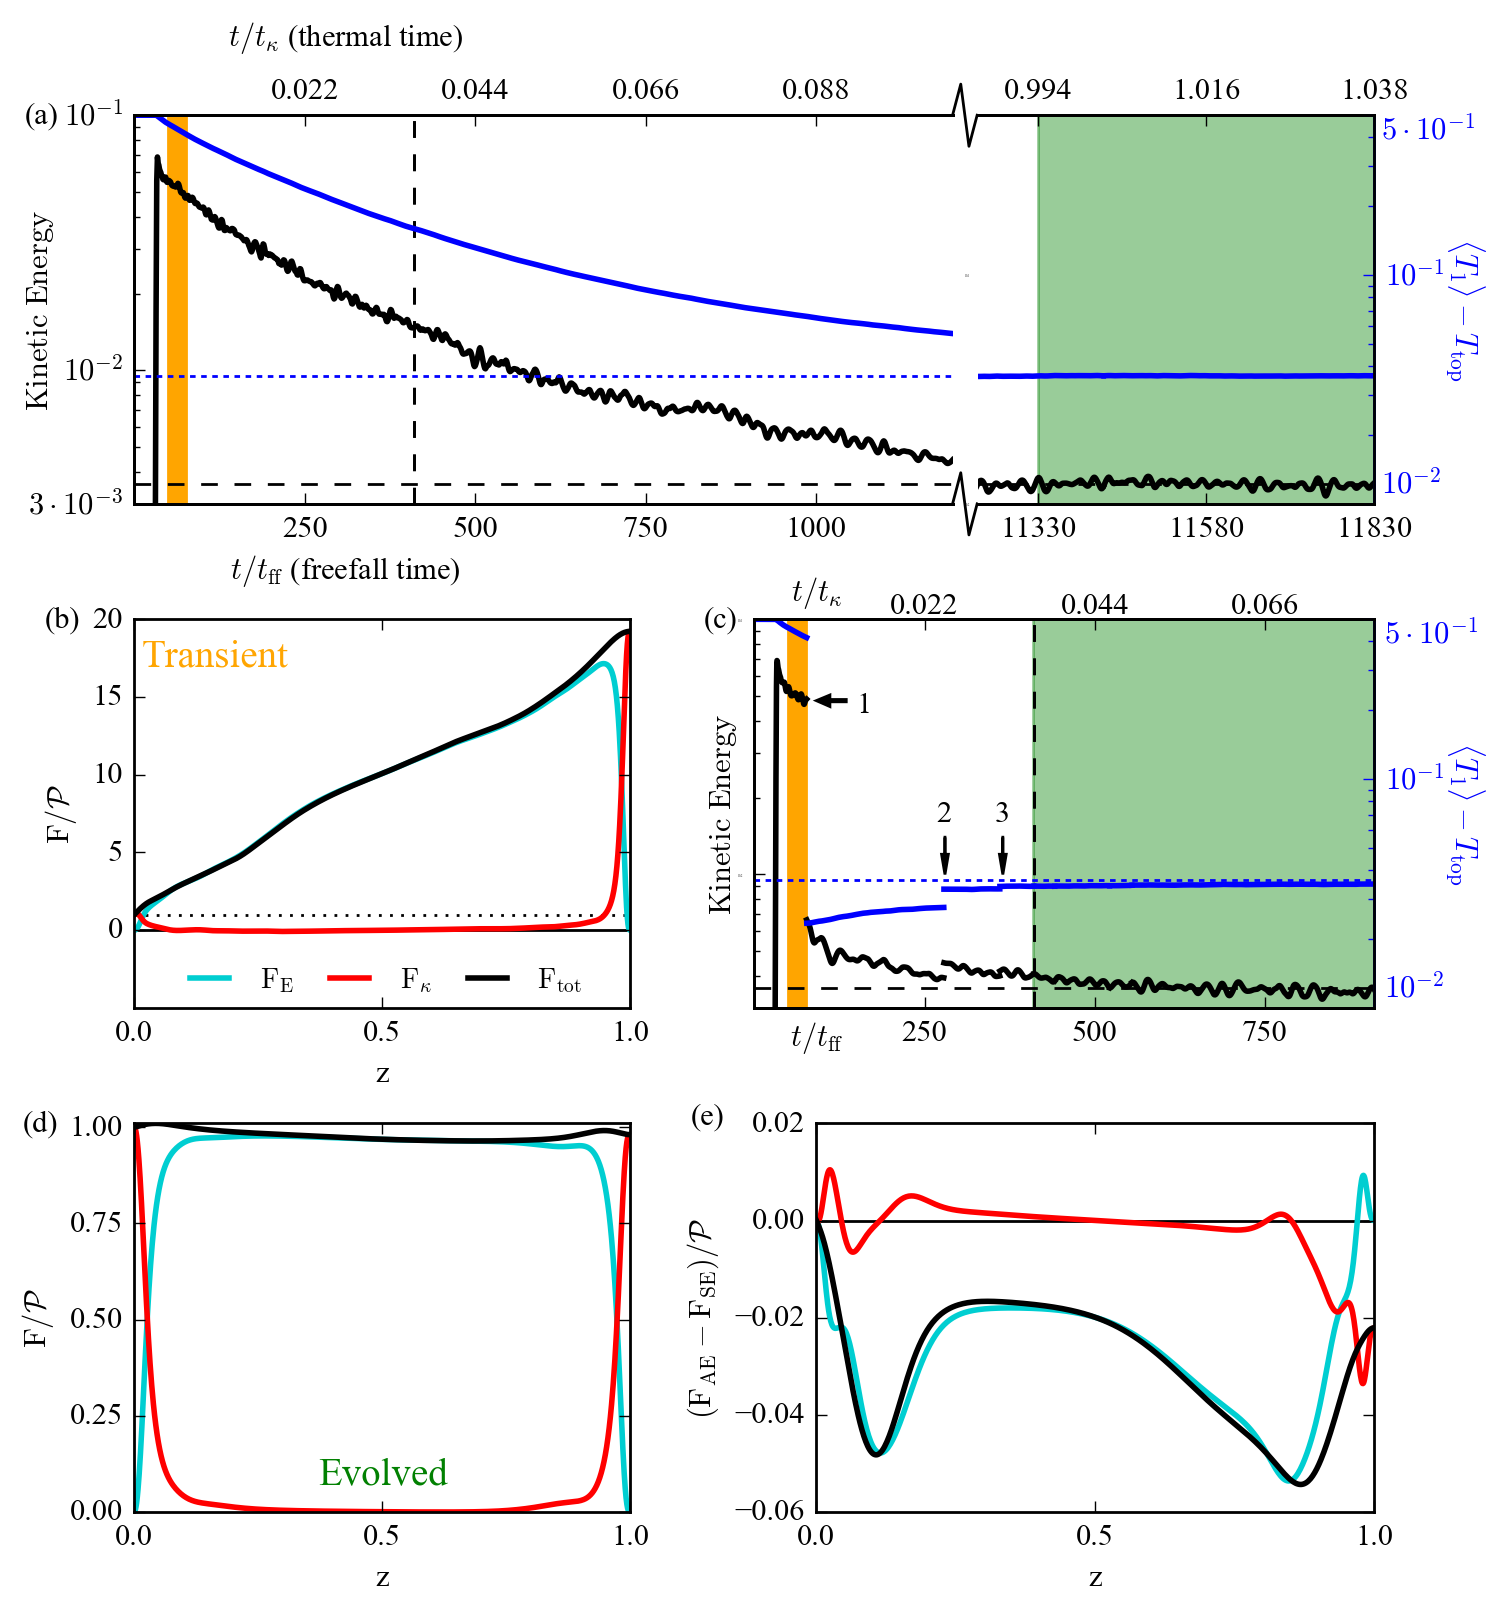
\includegraphics[width=\textwidth]{./figs/time_trace.png}
\caption{Traces of system energies vs. time for a long thermal rundown (a) and BVP convergence
(b) are shown for $S = 10^{4 + 2/3}$.  The horizontal extent of the subplots is set
such that one simulation time unit takes up an equal amount of paper space in (a) and (b). Volume averaged
kinetic energy is shown in black, and the volume averaged temperature with the top value removed, is shown
in red.
The dashed vertical line on (a) represents the time at which averaging begins in the BVP solution in (b),
and the horizontal dashed lines show the equilibrium value of the energies. The blue vertical lines represent
the beginning of the time-averaging window.
(c) System fluxes early in the run (the orange highlights in (a)) are shown.  
Black is the sum of the flux, purple
is the convective flux, and red is the conductive flux.
(d) Fluxes in the converged rundown IVP compared to the converged BVP.  The sum of flux is shown in
black \& grey, the convective flux is shown in purple \& pink, and the conductive flux is shown in red \& orange.
(e) The differences between the BVP and rundown fluxes is shown.  While not in perfect agreement, 
the BVP fluxes deviate from the rundown fluxes by only a few percent of the total flux, and
are much closer to the converged state than the initial fluxes, as in (c).
\label{fig:time_trace} }
\end{figure}

It is reasonable to assume that convection will evolve the mean temperature profile that
drives it over the course of a thermal diffusion time, $t_\chi = \mathcal{P}^{-1}$. Thus, as Ra
increases, the timescale for achieving a thermally converged mean temperature profile becomes intractable.
This prohibitively long thermal timescale in an Initial Value Problem (IVP)
can be skipped by coupling the IVP with a simple Boundary Value Problem
(BVP) solve. By using information about the convecting dynamical state of an unconverged solution,
a BVP can be used to solve for the evolved system state.
A comparison of a simulation running for the thermal timescale, and another where a BVP is used
to fast-forward atmospheric evolution, are shown in Fig \ref{fig:time_trace}a\&b.

The Boussinesq BVP in essence contains equations of hydrostatic balance and thermal equilibrium,
\begin{gather}
\frac{\partial}{\partial z}\angles{\varpi} - \angles{T_1}\hat{z} = \angles{\bm{u}\times\bm{\omega}},
	\label{eqn:bouss_BVP_momentum}
\\
\frac{\partial}{\partial z}\angles{wT_1} - \mathcal{P}\frac{\partial^2}{\partial z^2} \angles{T_1} = 0,
	\label{eqn:bouss_BVP_energy}
\end{gather}
where $\angles{A}$ represents a time- and horizontally averaged profile of the quantity $A$.  
These
equations arise from assuming that the atmosphere is in a steady state ($\partial_t \rightarrow 0$),
then taking time and horizontal averages of Eqns (\ref{eqn:bouss_momentum}\&\ref{eqn:bouss_energy}) and
neglecting terms that vanish due to the symmetry of the problem.
Convective flows
are perturbations around a thermal profile defined by these equations in the proper evolved, statistically stationary state.

Under eqns (\ref{eqn:bouss_BVP_momentum}\&\ref{eqn:bouss_BVP_energy}), 
the thermal structure ($\angles{T_1}$, $\angles{\varpi}$) of the atmosphere is fully determined by the specification
of two profiles: the convective flux, $F_{conv} = \angles{w T_1}$, and the nonlinear advection, $\angles{\bm{u}\times\bm{\omega}}$.  
If these profiles are known, then 
solving for $\angles{T_1}$ and
$\angles{\varpi}$ depends only upon the choice of boundary conditions.

By definition, the profile of $F_{\text{conv}}$ is not in a time stationary state early in the IVP.  
In fact, as the atmosphere approaches the
isotherm specified by the upper (fixed $T$) boundary condition, the motions display an asymmetric flux as energy
leaks through the upper boundary condition (Fig. \ref{fig:time_trace}c) in order to reach a lower temperature state.
In order to construct the evolved convective flux from the current fluxes in the atmosphere,
we assume that the atmospheric dynamics have properly developed the thickness of the boundary layers.
In other words, if we know the quantities $F_{\text{conv}}$, $F_{\text{cond}} = \angles{-P \partial_z T}$,
and $F_{\text{tot}} = F_{\text{conv}} + F_{\text{cond}}$, we assume that the profiles
\begin{equation}
f_{\text{conv}}(z) = \frac{F_{\text{conv}}}{F_{\text{tot}}},\qquad
f_{\text{cond}}(z) = \frac{F_{\text{cond}}}{F_{\text{tot}}}
\label{eqn:bvp_ratios}
\end{equation}
early in the evolution are the same as they will be in the final steady state solution. By definition, the
evolved total flux through the atmosphere must be the same as the flux entering the atmosphere at the
bottom boundary, $F_{\text{tot, steady}} = F_{\text{bot}}$.  The proper convective flux profile to use in
Eqn. (\ref{eqn:bouss_BVP_energy}) is then 
$\angles{w T_1}_{\text{steady}} = F_{\text{tot, steady}} \cdot f_{\text{conv}}$.  

In order to carry the converged amount of flux appropriately, 
the velocity field and temperature fluctuations in the system must be scaled by a quantity
$\xi(z) = \angles{w T_1}_{\text{steady}}/\angles{w T_1}$.  Thus, we multiply the velocities
and the thermal fluctuations, $T - \angles{T}$, by $\sqrt{\xi}$, such that the product of all fluctuations
(which carry the convective flux) are diminished by a factor of $\xi$.  This also means that
$\angles{\bm{u}\times\bm{\omega}}_{\text{steady}} = \xi \angles{\bm{u}\times\bm{\omega}}$. Once these profiles
are appropriately adjusted, they can be used in the BVP solve to find $\angles{T}$ and $\angles{\varpi}$.

In general, the BVP solve is completed in the following steps:
\begin{enumerate}
\item Run the convective IVP. Once the convection achieves a volume-averaged Re of $\sqrt{\text{Ra}/\text{Ra}_{\text{crit}}}$,
wait for 50 freefall time units.  
\item Start taking the averages of $F_{\text{conv}}$, $F_{\text{tot}}$, and $\angles{\bm{u} \times \bm{\omega}}$, waiting either
30 freefall time units or until the average profiles change by no more than 1 part in 1000 on a
given timestep, whichever is a more difficult criterion. This ensures that
the profiles being used in the BVP are steady and smooth, and that they sample the full behavior of the convection.
\item Construct $\angles{w T_1}_{\text{steady}}$, $\xi$, and $\angles{\bm{u}\times\bm{\omega}}_{\text{steady}}$
from the flux profiles.
\item Solve for $\angles{T_1}$ and \angles{\varpi} of the
evolved state.  Adjust the mean profiles in the IVP.
\item Multiply the velocity field and the fluctuations in $T_1$ about its horizontal average by $\sqrt{\xi}$ in the IVP. 
\item Continue running the IVP for freefall 50 time units to allow for the velocities to equilibrate to their new background state.
\item Repeat steps 2-6 to complete a second BVP and get closer to the right solution now that we
are far from the very unstable transient period.
\item Take averages for the amount of time specified for the given run in Appendix \ref{section:appendix_table}.
\end{enumerate}

\subsection{Numerics}
We utilize the 
Dedalus\footnote{\url{http://dedalus-project.org/}} 
pseudospectral framework \cite{burns&all2016} to time-evolve  
(\ref{eqn:incompressible})-(\ref{eqn:bouss_energy}) 
using an implicit-explicit (IMEX), third-order, four-step 
Runge-Kutta timestepping scheme RK443 \cite{ascher&all1997}.  
The linear terms (on the LHS of the equations) are solved implicitly,
while the nonlinear terms (RHS) are explicitly solved.
The temperature field is decomposed as $T = T_0(z) + T_1(x, y, z, t)$
and the velocity is $\bm{u} = w\bm{\hat{z}} + u\bm{\hat{x}} + v\bm{\hat{y}}$.
In our 2D runs, $v = 0$.
Variables are time-evolved on a dealiased Chebyshev (vertical)
and Fourier (horizontal, periodic) domain in which the
physical grid dimensions are 3/2 the size of the coefficient grid.  

As initial conditions, we fill $T_1$ with
random white noise whose magnitude is $10^{-6}(\text{Ra Pr})^{-1/2}$.
This ensures that the initial perturbations are much smaller than the
evolved convective temperature perturbations, even at large Ra.
We filter this noise spectrum in coefficient space, 
such that only the lower 25\% of the coefficients
have power.

\section{Results}
While Fig. \ref{fig:time_trace} shows us that the post-BVP and post-rundown solutions
exhibit similar system energies and fluxes, it is important to examine other aspects of
the evolved solution. The BVP mainly serves to adjust the thermodynamic state of the solution;
in \RB convection, this means that the evolved temperature profile is a good measure of whether
or not the BVP achieves the proper solution.

\begin{figure}[t]
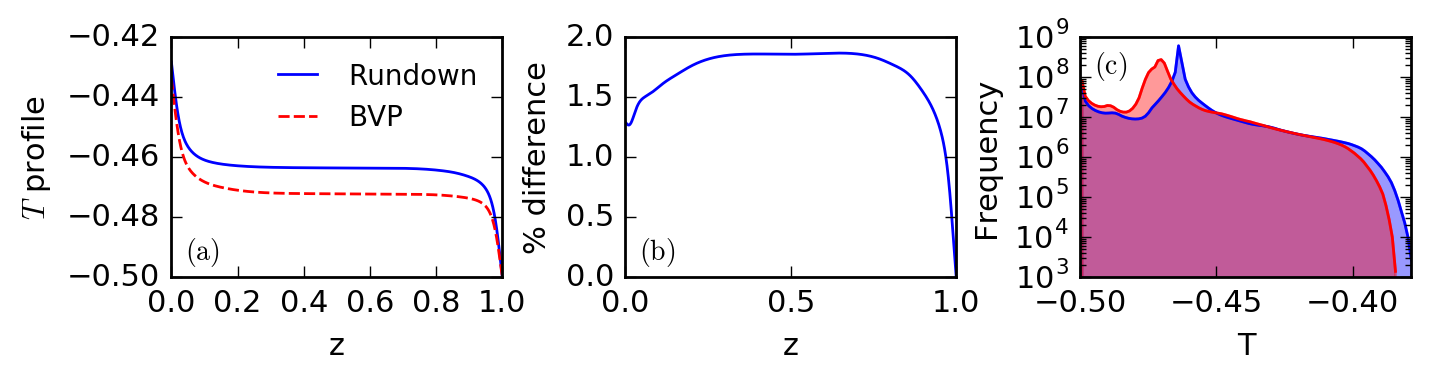
\includegraphics[width=\textwidth]{./figs/temp_comparison.png}
\caption{Comparisons of the evolved thermodynamic states of a BVP solution and a long IVP rundown at
$S = 10^{4 + 2/3}$ are shown.  (a) Evolved temperature profiles, as a function of height.
(b) The percentage difference between the temperature profiles (as shown in (a)), as a function of height.
(c) Probability distributions of point-by-point measurements of $T$ throughout the two domains over the
averaging windows are shown.  The cumulative distribution functions are overplotted and the maximum
difference between them in 0.0407. This difference arises due to the imperfect alignment of the
mean domain temperatures, but it is clear that otherwise the statistics are quite similar.
\label{fig:temp_comparison} }
\end{figure}


The temperature profiles of a 2D run at $S = 10^{4 + 2/3}$ 
for both the BVP solve and the long rundown are shown in
Fig. \ref{fig:temp_comparison}a.  While they are not perfectly aligned they are within less than
0.25\% of each other throughout the depth of the atmosphere, as shown in Fig. \ref{fig:temp_comparison}b.
While the mean temperature profile is interesting, the point-by-point fluctuations in the
temperature are what lead to convective transport, and thus examining the spread of temperature
and the allowed values that it can take are important to characterizing the system.  As seen
in Fig. \ref{fig:temp_comparison}c, aside from the noticeable difference in the mode of the
temperatures, the two runs exhibit largely the same spread of temperatures.
(AUTHOR NOTE: we aren't quite sure how to do a KS test properly here, but we can at least
list the KS statistic -- currently this is in the caption.)

In addition to examining the thermodynamics of the solutions, we are especially interested in
determining if the post-BVP solution appropriately captures key features of the nonlinear dynamics.
We show point-by-point probability distributions of the horizontal velocity, vertical velocity,
and nonlinear transport in Fig. \ref{fig:pdf_comparison}.  All of these measures have a sharp
peak at zero due to the no-slip, impenetrable boundary conditions and the denser grid sampling
near the boundaries of our Chebyshev grid.  Regardless, we see that the velocities of the 
two solutions are largely consistent.  The nonlinear transport in Fig. \ref{fig:pdf_comparison}c
shows that the rundown solution experiences a larger number of energetic, extreme events,
but the BVP displays a larger number of moderately energetic events than the IVP (as
evidenced by the differences in the cumulative distribution functions).

\begin{figure}[b]
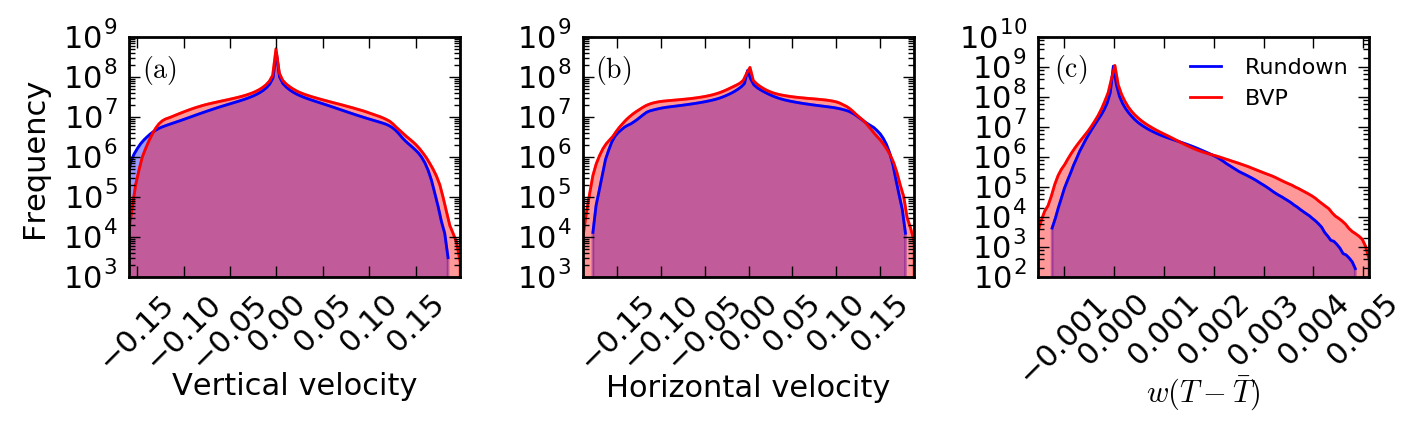
\includegraphics[width=\textwidth]{./figs/pdf_comparison.png}
\caption{Probability distribution functions of the vertical velocity (a), horizontal velocity (b), and nonlinear
vertical transport (c) are shown for a 2D run at $S = 10^{4 + 2/3}$.  We sample flows every 0.1 time units for 500 freefall
times, and include the flows at all points on the grid at each of these samples in these distributions.  All
distributions are biased by the no-slip, impenetrable boundary conditions, coupled with the dense spacing of our
Chebyshev grids near the boundaries, so there is a large peak around zero. 
The cumulative distribution function is overplotted on each plot, with a maximum difference of
(a) 0.027, (b) 0.0061, and (c) 0.035. There is an excess of higher-flux carrying
elements in the BVP solution than in the IVP rundown, despite the rundown's distribution
having more powerful, rare events.
\label{fig:pdf_comparison} }
\end{figure}


The goodness of this method has been tested across a broad range of supercriticality.  We have
examined both Rundown and BVP solutions in the range $S = [10^{1/3}, 10^5]$ in 2D and
$S = [10^1, 10^4]$ in 3D.  We have also further explored up to $S = 10^6$
(AUTHOR NOTE: we're going up to $10^8$ in 2D right now, need to mention this is state of
the art and give refs).
We show the volume averaged Nusselt number, RMS Reynolds number, and mean temperature in
the evolved BVP solutions in in Fig. \ref{fig:parameter_space_comparison}a-c.
The relative error of the BVP measurements of these values is compared to the IVP
measurements for these values in Fig. \ref{fig:parameter_space_comparison}d-f.

In Fig. \ref{fig:parameter_space_comparison}a, we show the Nusselt number scaling in 2D and
3D.  We use a classic definition of the Nusselt number
to measure the heat transport in these systems, where
\begin{equation}
\text{Nu} = \frac{\angles{F_{\text{conv}} + F_{\text{cond}}}}{\angles{F_{\text{cond, ref}}}}
 = \frac{\angles{wT - (\text{Ra Pr})^{-1/2}\grad T}}{\angles{- (\text{Ra Pr})^{-1/2} \grad T}}.
\end{equation}
At small values of $S$, we achieve a steady state solution with a clear value of Nu.  Near
$S \sim 10^3$, our simulations begin to achieve a horizontally oscillatory state.  Due to the
use of no-slip boundaries, these states never give way to full scale shearing states, but they
do reduce the overall heat transport through the system and cause the systems to oscillate between
periods of high- and low- heat transport.  The vertical lines represent the standard deviation 
of Nu associated with these oscillations, while the error bars show the drift of the mean
value of Nu over the averaging window.  We find that $\text{Nu} \propto \text{Ra}^{1/5}$,
a weaker scaling law than that seen in traditional \RB convection \cite{johnston&doering2009},
but similar to that seen in shearing states [cite Goluskin].
(AUTHOR NOTE: Ben, I think this is entirely because of the oscillatory states.  I wonder what
would happen if we included viscous fluxes...)

In Fig. \ref{fig:parameter_space_comparison}b, we measure the rms Reynolds number, where
$\text{Re} = \angles{|\bm{u}|} / \mathcal{R}$.  We find that this scales roughly as
$\text{Re} \propto \text{Ra}^{0.45}$.

In Fig. \ref{fig:parameter_space_comparison}c, we measure the volume averaged 
temperature of our solution, then subtract out the value at the upper (fixed $T$) boundary.
If the atmosphere were perfectly isothermal, this value would be exactly zero.  Thus, this is
a measure of the temperature jump across the boundary layers, and it provides insight both
into whether or not the temperature profiles of two runs are the same and into whether
the fluxes through the two systems are the same (it is in some ways an alternate measure of Nu
[cite King 2009 supp materials]).
We find that this measure is $\propto \text{Ra}^{-1/5}$, approaching zero, as expected.

For each of these measurements, the BVP achieves the same value as the IVP to
within about 3\% (Fig. \ref{fig:parameter_space_comparison}d-f).  This is good agreement,
and the residuals have a scattered distribution of positive and negative values, indicating
that the method is not biased towards the wrong answer in a clear manner.

\begin{figure}[t]
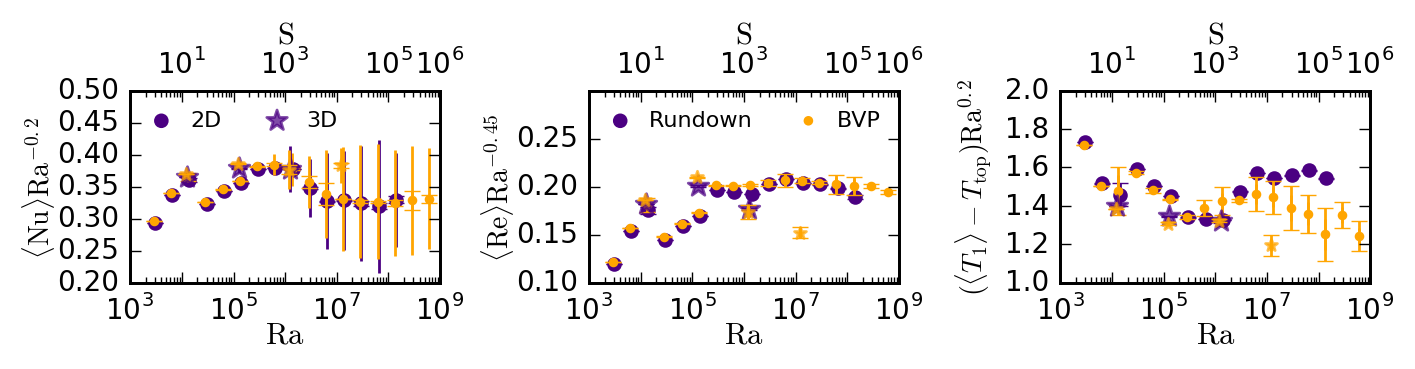
\includegraphics[width=\textwidth]{./figs/parameter_space_comparison.png}
\caption{Scaling plots are shown for the Nusselt number (a), the
Reynolds number (b), and the volume-averaged temperature (c).  
Symbols represent the mean value of
a measurement, vertical lines represent the standard deviation of the measurement over the
time window, and error bars represent the shift in the mean value over the window.
(a) Nu, which measures heat transport, scales roughly like $Ra^{1/5}$, and above Ra$\geq 10^6$,
simulations display horizontally oscillating plumes which have oscillating periods of high transport
and low transport.  The mean value is marginally diminished as a result, and the variance of Nu with time
is large. (b) Re, which measures the level of turbulence in the evolved solution, scales as
Ra$^{0.45}$ in 2D and is not distinctly different in 3D. (c) The average temperature flucutation, minus the top
temperature, which is a scalar measure of the final average thermodynamic state and should approach zero
in the limit of infinitely large Ra.
The temperature profile is slow to adjust, and differences between
BVP solutions and rundown solutions are quite easy to pick out in this measure. (d-f)
Relative error is shown between the BVP and IVP measurements of Nu (d), Re (e), and the
mean temperature (f). The grey box indicates the region in which only BVP runs were
carried out due to computational expense.
\label{fig:parameter_space_comparison} }
\end{figure}


\section{Discussion \& Conclusions}
\label{sec:results}
The method presented here is a first step towards taking meaningful measurements
of highly turbulent convection on manageable, human timescales.  As demonstrated in Figs.
1-4, this BVP method quickly converges simulations to within a few percent of the true final
state. Furthermore, the total simulation time required to use the BVPs does not change drastically from
low $S$ to high $S$, so the main prohibition on high Ra states is the difficulty of timesteps becoming
increasingly small as turbulence increases.  Additionally, post-BVP, we generally see an increase of the
timestep size by nearly a factor of two due to the less intense driving of the near-converged state that
is achieved quickly.  

It is important to note that the measurements made in
this paper were generally done for short timescales (a few hundred buoyancy times) in
order to show the precise differences between the BVP solutions and the IVP solutions.
Where there are differences, the BVP solution is trending towards the IVP solution,
and if measurements were taken over long timescales (e.g., a thermal time), the
differences between the BVP solution and IVP solution would be negligible.

One major benefit of the BVP method used here is that it preserves the natural behavior of 
the convective solution (such as the horizontally oscillatory rolls
of high-Ra 2D states in Fig. \ref{fig:parameter_space_comparison}).
One frequently used method of measuring dynamics in high-Ra simulations is that of bootstrapping,
in which the converged solution of a low-Ra state is used as initial conditions for a higher-Ra
simulation.  While this method is powerful, it can be influenced by hysteresis effects,
and the steady rolls achieved at low Ra can result in an artifically over-stable high-Ra
roll solution.  The BVP method we present here uses random noise initial conditions which allows the
convective solution to naturally choose the dynamics.

Another benefit of our BVP method is that it can be easily extended to more complicated
configurations.  For example, to use this method in simulations of stratified compressible convection,
one need only adapt the BVP equations to the appropriate equations of hydrostatic equilibrium
and thermal equilibrium obtained by averaging the fully compressible, ideal gas
steady state momentum and energy equations \cite{anders&brown2017, lecoanet&all2014}.
In compressible convection, where the density is allowed to change,
it is also essential to conserve mass by adding boundary conditions on the integrated mas density at
the upper and lower boundaries, much as stellar structure codes do \cite{paxton&all2011}.

While we have not chosen to use them here, this BVP method can be extended to other boundary conditions.  
To solve for fixed temperature boundary conditions, the 
main difficulty is in finding the amount of flux through the system, $F_{\text{tot, steady}}$.
However, by knowing the averaged value of the conductive flux (from the boundary conditions)
and the ratios in Eqn. (\ref{eqn:bvp_ratios}), $F_{\text{tot, steady}}$ can be found.
In the case of
fixed flux boundary conditions, the temperature solution is degenerate.
However, using knowledge about the system -- such as the initial symmetry of the
RB state around $T = 0$, the final solution can be pegged onto the proper profile.

Future work will aim to apply the methods presented here to compressible systems,
internally heated systems, and systems with more complex forms of the conductive flux.


\begin{acknowledgments}
EHA acknowledges the support of the University of Colorado's George 
Ellery Hale Graduate Student Fellowship.
This work was additionally supported by  NASA LWS grant number NNX16AC92G.  
Computations were conducted 
with support by the NASA High End Computing (HEC) Program through the NASA 
Advanced Supercomputing (NAS) Division at Ames Research Center on Pleiades
with allocations GID s1647 and GID g26133.
\end{acknowledgments}


\appendix
\section{Table of Runs}
\label{section:appendix_table}
\begin{center}
\begin{tabularx}{\textwidth}{ X X X X X X X X X}
\hline															
$S$	&	Ra	&	nz	&	nx, ny	&	$t_{\text{therm}}$	&	$t_{\text{avg}}$	&	Nu$_{\text{rundown}}$	&	Nu$_{\text{BVP}}$	\\
\hline															
$10^{1/3}$	&	$2.79 \cdot 10^3$	&	32	&	128	&	$52.8$	&	100	&	(TBD)	&	(TBD)	\\
$10^{2/3}$	&	$6.01 \cdot 10^3$	&	32	&	128	&	$77.6$	&	100	&	--	&	--	\\
$10^1$	&	$1.30 \cdot 10^4$	&	32	&	128	&	$114$	&	100	&	--	&	--	\\
$10^{1 + 1/3}$	&	$2.79 \cdot 10^4$	&	32	&	128	&	$167$	&	100	&	--	&	--	\\
$10^{1 + 2/3}$	&	$6.01 \cdot 10^4$	&	32	&	128	&	$245$	&	100	&	--	&	--	\\
$10^2$	&	$1.30 \cdot 10^5$	&	64	&	256	&	$360$	&	100	&	--	&	--	\\
$10^{2 + 1/3}$	&	$2.79 \cdot 10^5$	&	64	&	256	&	$528$	&	100	&	--	&	--	\\
$10^{2 + 2/3}$	&	$6.01 \cdot 10^5$	&	64	&	256	&	$776$	&	100	&	--	&	--	\\
$10^3$	&	$1.30 \cdot 10^6$	&	128	&	512	&	$1.14 \cdot 10^3$	&	200	&	--	&	--	\\
$10^{3 + 1/3}$	&	$2.79 \cdot 10^6$	&	128	&	512	&	$1.67 \cdot 10^3$	&	500	&	--	&	--	\\
$10^{3 + 2/3}$	&	$6.01 \cdot 10^6$	&	256	&	1024	&	$2.45 \cdot 10^3$	&	500	&	--	&	--	\\
$10^4$	&	$1.30 \cdot 10^7$	&	256	&	1024	&	$3.60 \cdot 10^3$	&	500	&	--	&	--	\\
$10^{4 + 1/3}$	&	$2.79 \cdot 10^7$	&	256	&	1024	&	$5.28 \cdot 10^3$	&	500	&	--	&	--	\\
$10^{4 + 2/3}$	&	$6.01 \cdot 10^7$	&	256	&	1024	&	$7.76 \cdot 10^3$	&	500	&	--	&	--	\\
$10^5$	&	$1.30 \cdot 10^8$	&	512	&	2048	&	$1.14 \cdot 10^4$	&	500	&	--	&	--	\\
$10^{5 + 1/3}$	&	$2.79 \cdot 10^8$	&	512	&	2048	&	$1.67 \cdot 10^4$	&	500	&	--	&	--	\\
$10^{5 + 2/3}$	&	$6.01 \cdot 10^8$	&	512	&	2048	&	$2.45 \cdot 10^4$	&	500	&	--	&	--	\\
$10^6$	&	$1.30 \cdot 10^9$	&	1024	&	4096	&	$3.60 \cdot 10^4$	&	500	&	--	&	--	\\
\hline															
\end{tabularx}
\end{center}



\bibliography{biblio.bib}
\end{document}
